\documentclass[11pt,a4paper]{article}

% --- Codificación y tipografía ---
\usepackage[utf8]{inputenc}
\usepackage[T1]{fontenc}
\usepackage{lmodern}

% --- Diseño de página, tablas y gráficos ---
\usepackage[margin=2.3cm]{geometry}
\usepackage{array}
\usepackage{longtable}
\usepackage{booktabs}
\usepackage[table]{xcolor}
\usepackage{titlesec}
\usepackage{enumitem}
\usepackage{tcolorbox}
\usepackage{tikz}
\usetikzlibrary{arrows.meta, positioning, shapes.geometric, fit, backgrounds}
\usepackage{hyperref}

\hypersetup{
  colorlinks=true,
  linkcolor=teal!60!black,
  urlcolor=teal!60!black,
  pdftitle={Funcionamiento del proyecto Papaws},
  pdfauthor={Equipo Papaws}
}

% --- Colores corporativos aproximados del proyecto ---
\definecolor{moss}{HTML}{005F73}
\definecolor{moss2}{HTML}{0A9396}
\definecolor{mosslight}{HTML}{D7E8E6}
\definecolor{clay}{HTML}{BB3E03}
\definecolor{sun}{HTML}{EE9B00}
\definecolor{ink}{HTML}{2B2D31}
\definecolor{codebg}{HTML}{F4F6F6}

\titleformat{\section}{\Large\bfseries\color{moss}}{\thesection}{0.6em}{}
\titleformat{\subsection}{\large\bfseries\color{clay}}{\thesubsection}{0.6em}{}
\titleformat{\subsubsection}{\normalsize\bfseries\color{moss2}}{\thesubsubsection}{0.6em}{}

% --- Caja para rutas / código corto ---
\newtcbox{\rutabox}{on line, boxrule=0pt, boxsep=0pt, top=1pt, bottom=1pt,
  left=3pt, right=3pt, arc=2pt, colback=codebg, fontupper=\ttfamily\small}

% --- Caja de nota ---
\newtcolorbox{nota}{colback=mosslight, colframe=moss, boxrule=0.6pt,
  arc=2pt, left=6pt, right=6pt, top=4pt, bottom=4pt}

% --- Tipos de columna para tablas de endpoints ---
\newcolumntype{M}{>{\ttfamily\small}p{2.0cm}}   % método HTTP
\newcolumntype{P}{>{\ttfamily\small}p{6.0cm}}   % path
\newcolumntype{D}{p{6.3cm}}                       % descripción

\title{\textbf{\color{moss}Funcionamiento del proyecto Papaws}\\[0.3em]
\large Arquitectura de microservicios, servicios y flujo de datos}
\author{Equipo Papaws}
\date{\today}

\begin{document}

\maketitle

\begin{abstract}
\noindent
\textbf{Papaws} es un sistema de gestión para un refugio veterinario de animales
rescatados. Está construido como un conjunto de \textbf{microservicios} en
\texttt{ASP.NET Core} (.NET~10) con persistencia en \textbf{Apache Cassandra}, y
un \textbf{frontend} en \texttt{React + TypeScript + Vite}. Este documento explica
qué hace cada servicio, cómo están conectados entre sí, qué información muestra la
interfaz y cómo se despliega todo el conjunto. Para el detalle del modelo de datos
físico (tablas y claves de Cassandra) consúltese el documento complementario
\emph{Esquema de tablas en Cassandra}.
\end{abstract}

\tableofcontents
\vspace{1em}

% ===================================================================
\section{Visión general}
% ===================================================================

El sistema se divide en cuatro piezas desplegables independientes, más dos bases
de datos Cassandra:

\begin{itemize}[leftmargin=1.4em]
  \item \textbf{Pawpaws-Animales} (puerto \rutabox{8080}): gestiona
        \emph{rescatistas} y \emph{animales}. Es además el \textbf{emisor de los
        tokens de autenticación} (login) para todo el sistema.
  \item \textbf{Pawpaws-Consulta} (puerto \rutabox{8081}): gestiona
        \emph{consultas} veterinarias y sus catálogos asociados:
        \emph{veterinarios}, \emph{servicios} y \emph{productos} (inventario).
  \item \textbf{Pawpaws-Reportes} (puerto \rutabox{8082}): servicio de
        \emph{solo lectura} que agrega y combina datos de los otros dos servicios
        para producir reportes; no tiene base de datos propia.
  \item \textbf{Pawpaws-Front} (puerto \rutabox{5173} en desarrollo): la
        aplicación web de una sola página (SPA) que consume las tres APIs.
\end{itemize}

\begin{nota}
\textbf{Idea clave.} Cada microservicio es dueño de sus propios datos y de su
propio keyspace de Cassandra. Cuando un servicio necesita información de otro,
\emph{no} accede a su base de datos: hace una llamada HTTP a su API, reenviando el
token del usuario. Reportes es un caso especial: \emph{solo} habla por HTTP con
los otros dos y no almacena nada.
\end{nota}

% ===================================================================
\subsection{Diagrama de componentes}
% ===================================================================

\begin{center}
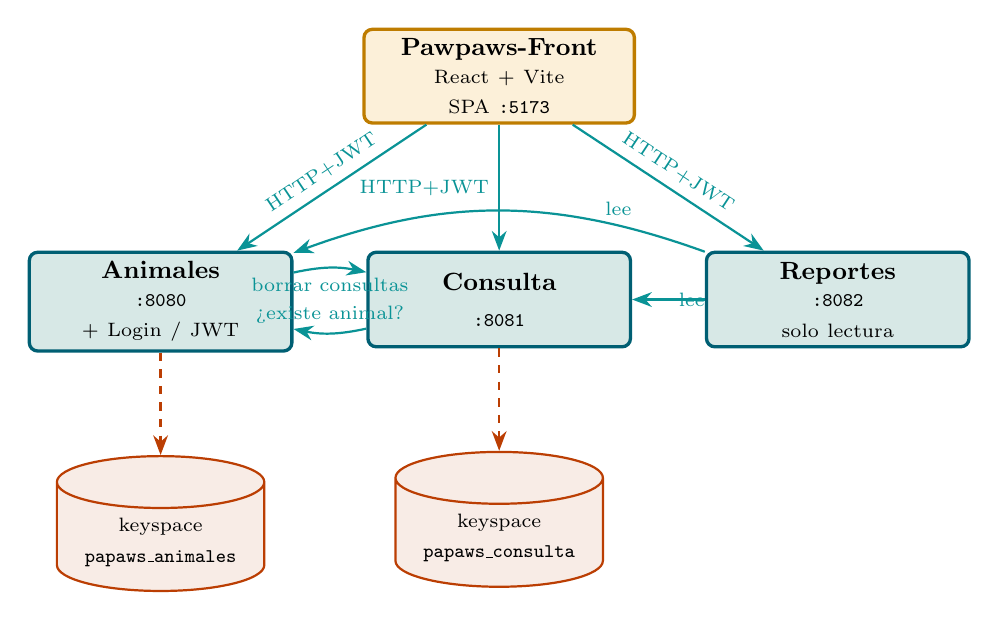
\begin{tikzpicture}[
  font=\small,
  servicio/.style={rectangle, rounded corners=3pt, draw=moss, very thick,
    fill=mosslight, text width=3.1cm, align=center, minimum height=1.2cm},
  db/.style={cylinder, shape border rotate=90, aspect=0.25, draw=clay,
    thick, fill=clay!10, text width=2.4cm, align=center, minimum height=1.4cm},
  front/.style={rectangle, rounded corners=3pt, draw=sun!80!black, very thick,
    fill=sun!15, text width=3.2cm, align=center, minimum height=1.1cm},
  http/.style={-{Stealth[length=2.5mm]}, thick, moss2},
  dbedge/.style={-{Stealth[length=2.5mm]}, thick, clay, dashed},
]

% Frontend
\node[front] (front) {\textbf{Pawpaws-Front}\\[2pt]\scriptsize React + Vite\\\scriptsize SPA \texttt{:5173}};

% Servicios
\node[servicio, below=1.6cm of front, xshift=-4.3cm] (anim) {\textbf{Animales}\\[2pt]\scriptsize \texttt{:8080}\\\scriptsize + Login / JWT};
\node[servicio, below=1.6cm of front] (cons) {\textbf{Consulta}\\[2pt]\scriptsize \texttt{:8081}};
\node[servicio, below=1.6cm of front, xshift=4.3cm] (rep) {\textbf{Reportes}\\[2pt]\scriptsize \texttt{:8082}\\\scriptsize solo lectura};

% Bases de datos
\node[db, below=1.3cm of anim] (dbA) {\scriptsize keyspace\\\texttt{papaws\_animales}};
\node[db, below=1.3cm of cons] (dbC) {\scriptsize keyspace\\\texttt{papaws\_consulta}};

% Aristas frontend -> servicios
\draw[http] (front) -- (anim) node[midway, sloped, above, font=\scriptsize]{HTTP+JWT};
\draw[http] (front) -- (cons) node[midway, left, font=\scriptsize]{HTTP+JWT};
\draw[http] (front) -- (rep) node[midway, sloped, above, font=\scriptsize]{HTTP+JWT};

% Servicio -> DB
\draw[dbedge] (anim) -- (dbA);
\draw[dbedge] (cons) -- (dbC);

% Comunicación entre servicios
\draw[http, bend left=12] (cons) to node[midway, above, font=\scriptsize]{¿existe animal?} (anim);
\draw[http, bend left=12] (anim) to node[midway, below, font=\scriptsize]{borrar consultas} (cons);
\draw[http] (rep) -- (cons) node[midway, right, font=\scriptsize]{lee} ;
\draw[http, bend right=20] (rep) to node[pos=0.2, above, font=\scriptsize]{lee} (anim);

\end{tikzpicture}
\end{center}

\noindent
\textit{Líneas continuas: llamadas HTTP (REST) con cabecera \texttt{Authorization:
Bearer <token>}. Líneas discontinuas: acceso del servicio a su keyspace de
Cassandra.}

% ===================================================================
\section{Tecnologías utilizadas}
% ===================================================================

\begin{center}
\begin{tabular}{>{\bfseries}p{3.2cm} p{10.5cm}}
\toprule
\rowcolor{moss}\textcolor{white}{\textbf{Capa}} & \textcolor{white}{\textbf{Tecnología}} \\
\midrule
Backend       & ASP.NET Core (.NET 10), controladores Web API, Swagger/OpenAPI. \\
Persistencia  & Apache Cassandra 4.1, driver \texttt{CassandraCSharpDriver}, \texttt{PreparedStatement}. \\
Autenticación & JWT (HMAC-SHA256) emitido por el servicio de Animales; validado por los tres servicios. \\
Frontend      & React 18, TypeScript, Vite, React Router, Tailwind CSS, Recharts (gráficos), lucide-react (iconos). \\
Infraestructura & Docker / Docker Compose; dos nodos Cassandra; healthchecks. \\
\bottomrule
\end{tabular}
\end{center}

% ===================================================================
\section{Pawpaws-Animales}
% ===================================================================

Es el servicio \textbf{central} y la puerta de entrada de la autenticación.

\subsection{Responsabilidades}
\begin{itemize}[leftmargin=1.4em]
  \item Administrar \textbf{rescatistas} (personas u organizaciones que rescatan
        animales) y los \textbf{animales} a su cargo.
  \item Emitir el \textbf{token JWT} de login que usa todo el sistema
        (\rutabox{POST /api/auth/login}).
  \item Mantener la coherencia al \textbf{eliminar} entidades: al borrar un animal
        ordena en cascada el borrado de sus consultas en el servicio de Consulta;
        al borrar un rescatista, reasigna sus animales a otro (por defecto al
        rescatista interno \emph{«Refugio»}).
\end{itemize}

\subsection{Estructura interna}
El servicio sigue una arquitectura en capas clásica:
\begin{itemize}[leftmargin=1.4em]
  \item \textbf{Controllers} — exponen los endpoints REST y aplican autorización por rol.
  \item \textbf{Services} — contienen la lógica de negocio y las consultas a Cassandra
        mediante \texttt{PreparedStatement}.
  \item \textbf{Models} — entidades de dominio (\texttt{Animal}, \texttt{Rescatista}).
  \item \textbf{DTOs} — objetos de entrada/salida de la API (separados del modelo).
  \item \textbf{Data/CassandraSchema} — crea el keyspace y las tablas al arrancar
        (idempotente, con migraciones \texttt{ALTER ... IF NOT EXISTS}).
  \item \textbf{Security} — opciones de JWT, usuarios semilla y roles.
  \item \textbf{Common} — manejador global de excepciones, healthcheck de Cassandra,
        mappers y paginación.
\end{itemize}

\subsection{Datos que administra}
\begin{itemize}[leftmargin=1.4em]
  \item \textbf{Rescatista}: nombre, teléfono, correo, organización, zona de
        operación; banderas \texttt{activo} (borrado lógico) y \texttt{oculto}
        (el «Refugio» interno no se muestra en listados).
  \item \textbf{Animal}: nombre, especie, peso actual, fecha de ingreso y el
        rescatista asociado. Se almacena en dos tablas desnormalizadas
        (\texttt{animales\_by\_id} y \texttt{animales\_by\_rescatista}) para poder
        consultarlo por ambas claves.
\end{itemize}

\subsection{Endpoints principales}
\begin{center}
\begin{longtable}{M P D}
\rowcolor{moss}\textcolor{white}{\textbf{Método}} & \textcolor{white}{\textbf{Ruta}} & \textcolor{white}{\textbf{Descripción}} \\
\midrule \endhead
POST   & /api/auth/login            & Autentica y devuelve el token JWT (anónimo). \\
GET    & /api/rescatistas           & Lista rescatistas activos (paginado). \\
POST   & /api/rescatistas           & Crea un rescatista. \\
PUT    & /api/rescatistas/\{id\}      & Actualiza un rescatista. \\
DELETE & /api/rescatistas/\{id\}      & Baja lógica; reasigna sus animales (\texttt{?reasignarA=}). \\
GET    & /api/animales              & Lista animales (paginado). \\
GET    & /api/animales/\{id\}         & Obtiene un animal (lo usa Consulta y Reportes). \\
GET    & /api/animales/rescatista/\{id\} & Animales de un rescatista. \\
POST   & /api/animales             & Crea un animal. \\
PUT    & /api/animales/\{id\}        & Actualiza un animal. \\
DELETE & /api/animales/\{id\}        & Borra el animal y, en cascada, sus consultas. \\
GET    & /health                   & Healthcheck (estado de Cassandra). \\
\end{longtable}
\end{center}

% ===================================================================
\section{Pawpaws-Consulta}
% ===================================================================

Gestiona el núcleo clínico del refugio: las consultas veterinarias y sus catálogos.

\subsection{Responsabilidades}
\begin{itemize}[leftmargin=1.4em]
  \item Administrar \textbf{veterinarios}, \textbf{servicios} (procedimientos con
        precio y duración) y \textbf{productos} (inventario con \texttt{stock}).
  \item Gestionar el \textbf{ciclo de vida de una consulta}: creación, edición,
        reprogramación, cambio de estado, registro de diagnóstico y de productos
        usados, y cancelación.
  \item Validar contra el servicio de Animales que el \textbf{animal exista} antes
        de crear una consulta (llamada HTTP, no acceso directo a la otra BD).
\end{itemize}

\subsection{Estados de una consulta}
Una consulta transita por una máquina de estados controlada:
\begin{center}
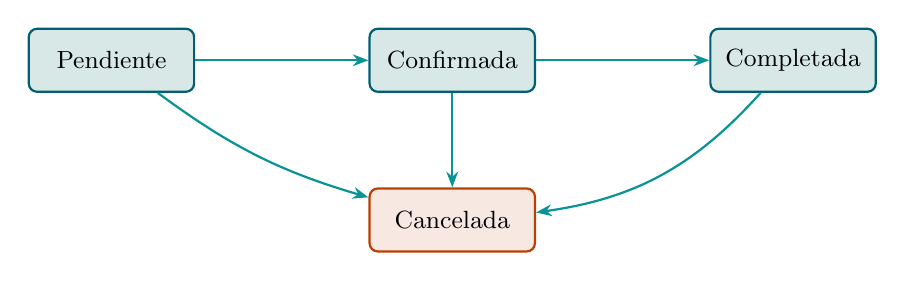
\begin{tikzpicture}[font=\small, node distance=2.2cm,
  estado/.style={rectangle, rounded corners=3pt, draw=moss, thick,
    fill=mosslight, minimum width=2.1cm, minimum height=0.8cm},
  cancel/.style={rectangle, rounded corners=3pt, draw=clay, thick,
    fill=clay!12, minimum width=2.1cm, minimum height=0.8cm},
  tr/.style={-{Stealth[length=2mm]}, thick, moss2}]
  \node[estado] (pen) {Pendiente};
  \node[estado, right=of pen] (con) {Confirmada};
  \node[estado, right=of con] (com) {Completada};
  \node[cancel, below=1.2cm of con] (can) {Cancelada};
  \draw[tr] (pen) -- (con);
  \draw[tr] (con) -- (com);
  \draw[tr] (pen) to[bend right=10] (can);
  \draw[tr] (con) -- (can);
  \draw[tr] (com) to[bend left=20] (can);
\end{tikzpicture}
\end{center}
\noindent
Reglas relevantes: una consulta \textbf{Cancelada} no cambia de estado; una
\textbf{Completada} solo puede cancelarse. Registrar un diagnóstico o productos
marca la consulta como \textbf{Completada}. Al \textbf{cancelar}, los productos que
se habían registrado se \textbf{devuelven al stock} automáticamente.

\subsection{Gestión de inventario}
El registro de productos usados es transaccional en su validación: primero se
valida \emph{todo} (existencia, baja lógica y stock suficiente) y solo después se
descuenta el stock, evitando descuentos a medias. Las cantidades se acumulan por
producto para no perder registros previos.

\subsection{Endpoints principales}
\begin{center}
\begin{longtable}{M P D}
\rowcolor{moss}\textcolor{white}{\textbf{Método}} & \textcolor{white}{\textbf{Ruta}} & \textcolor{white}{\textbf{Descripción}} \\
\midrule \endhead
GET    & /api/veterinarios          & Catálogo de veterinarios. \\
GET    & /api/servicios             & Catálogo de servicios. \\
GET    & /api/productos             & Inventario de productos. \\
PUT    & /api/productos/\{id\}/stock  & Establece el stock de un producto. \\
GET    & /api/consultas             & Lista consultas (liviano). \\
GET    & /api/consultas/\{codigo\}    & Detalle de consulta (con servicios y productos). \\
GET    & /api/consultas/animal/\{id\} & Consultas de un animal. \\
GET    & /api/consultas/veterinario/\{id\} & Consultas de un veterinario. \\
POST   & /api/consultas             & Crea una consulta (valida animal en Animales). \\
PUT    & /api/consultas/\{codigo\}/estado     & Cambia el estado. \\
PUT    & /api/consultas/\{codigo\}/reprogramar & Cambia la fecha/hora. \\
PUT    & /api/consultas/\{codigo\}/diagnostico & Registra diagnóstico (completa). \\
POST   & /api/consultas/\{codigo\}/productos   & Registra productos usados (descuenta stock). \\
DELETE & /api/consultas/\{codigo\}    & Cancela/elimina la consulta (restaura stock). \\
DELETE & /api/consultas/animal/\{id\} & Borrado en cascada (lo invoca Animales). \\
\end{longtable}
\end{center}

% ===================================================================
\section{Pawpaws-Reportes}
% ===================================================================

Servicio de \textbf{agregación de solo lectura}. No tiene base de datos: actúa como
un \emph{Backend-for-Frontend} de reportes que consulta por HTTP a Animales y a
Consulta, combina los resultados y los devuelve ya formateados.

\subsection{Cómo funciona}
\begin{itemize}[leftmargin=1.4em]
  \item Define dos clientes HTTP tipados: \texttt{AnimalesClient} (apunta a
        \rutabox{:8080}) y \texttt{ConsultaClient} (apunta a \rutabox{:8081}).
  \item \texttt{ReporteService} orquesta las llamadas: por ejemplo, para el reporte
        «consultas por animal» obtiene primero el animal de Animales y luego sus
        consultas de Consulta, y compone un único DTO de respuesta.
  \item Los DTOs de entrada externos viven en \rutabox{DTOs/Externos} y los DTOs de
        salida del reporte (C1\ldots C19) en \rutabox{DTOs/Reportes}.
\end{itemize}

\subsection{Catálogo de reportes}
El servicio expone alrededor de 18 reportes numerados (C1--C19). Algunos ejemplos:

\begin{center}
\begin{tabular}{>{\ttfamily\small}l p{10.5cm}}
\toprule
\rowcolor{moss}\textcolor{white}{\textbf{Cód.}} & \textcolor{white}{\textbf{Reporte}} \\
\midrule
C1  & Datos de un rescatista por id. \\
C2  & Animales de un rescatista. \\
C3  & Animales por especie. \\
C4  & Consultas de un animal. \\
C5  & Consultas de un veterinario. \\
C6  & Detalle completo de una consulta. \\
C7  & Consultas por estado. \\
C8  & Servicios usados en una consulta. \\
C9  & Productos usados en una consulta. \\
C10 & Productos ordenados por stock. \\
C13 & Veterinarios por especialidad. \\
C16 & Consultas por fecha. \\
C17 & Animales por nombre. \\
C19 & Rescatistas por zona. \\
\bottomrule
\end{tabular}
\end{center}

\noindent
La interfaz consume estos reportes en \rutabox{/api/reportes/...} y los muestra como
tablas y gráficos.

% ===================================================================
\section{Pawpaws-Front (interfaz web)}
% ===================================================================

SPA en React que es lo único que ve el usuario. Se comunica con las tres APIs.

\subsection{Páginas y qué muestran}
\begin{center}
\begin{tabular}{>{\bfseries}p{3.0cm} p{10.7cm}}
\toprule
\rowcolor{moss}\textcolor{white}{\textbf{Página}} & \textcolor{white}{\textbf{Contenido}} \\
\midrule
Login        & Formulario de acceso; obtiene el token de Animales. \\
Dashboard    & Resumen general / inicio. \\
Rescatistas  & Listado y CRUD de rescatistas (con reasignación al borrar). \\
Animales     & Listado y CRUD de animales; filtrado por rescatista. \\
Veterinarios & Catálogo de veterinarios (módulo consultas). \\
Servicios    & Catálogo de servicios. \\
Productos    & Inventario y ajuste de stock. \\
Consultas    & Listado de consultas y creación. \\
ConsultaDetalle & Detalle de una consulta: estado, diagnóstico, servicios y productos usados. \\
Reportes     & Reportes C1--C19 visualizados con tablas y gráficos (Recharts). \\
\bottomrule
\end{tabular}
\end{center}

\subsection{Organización del código}
\begin{itemize}[leftmargin=1.4em]
  \item \rutabox{api/client.ts} — capa HTTP base: añade el token, gestiona errores y
        el \texttt{401} (cierra sesión automáticamente).
  \item \rutabox{api/endpoints.ts} — funciones tipadas por dominio
        (\texttt{rescatistasApi}, \texttt{consultasApi}, \texttt{reportesApi}\ldots).
  \item \rutabox{auth/} — \texttt{AuthContext} (estado de sesión) y \emph{guards}
        de ruta (\texttt{ProtectedRoute}, \texttt{RoleRoute}).
  \item \rutabox{pages/} — una página por módulo; \rutabox{components/} — UI
        reutilizable; \rutabox{hooks/} — \texttt{useFetch}; \rutabox{types/} —
        tipos compartidos con el backend.
\end{itemize}

\subsection{Enrutamiento y protección por rol}
Las rutas están envueltas en \texttt{ProtectedRoute} (exige sesión) y el módulo de
consultas, además, en \texttt{RoleRoute} (solo \emph{Administrador} y
\emph{EncargadoConsultas}). El token se guarda en \texttt{localStorage}; si una API
devuelve \texttt{401}, la app emite un evento \texttt{papaws:unauthorized} y vuelve
al login.

% ===================================================================
\section{Autenticación y autorización}
% ===================================================================

\subsection{Flujo del token}
\begin{enumerate}[leftmargin=1.6em]
  \item El usuario hace login contra \rutabox{POST :8080/api/auth/login}.
  \item Animales valida las credenciales contra una lista de \textbf{usuarios
        semilla} (modelo simple con contraseña genérica de desarrollo) y firma un
        \textbf{JWT} con HMAC-SHA256.
  \item El token incluye el \texttt{rol} del usuario y caduca (480 min por defecto).
  \item El frontend lo almacena y lo envía como \rutabox{Authorization: Bearer ...}
        en cada llamada.
  \item Los \textbf{tres} servicios validan el mismo token con la \textbf{misma
        clave} (\texttt{Auth:Jwt:Key}); solo Animales lo \emph{emite}.
\end{enumerate}

\subsection{Roles}
\begin{center}
\begin{tabular}{>{\bfseries}p{4.2cm} p{9.5cm}}
\toprule
\rowcolor{moss}\textcolor{white}{\textbf{Rol}} & \textcolor{white}{\textbf{Permisos}} \\
\midrule
Administrador        & Acceso completo a todos los módulos. \\
EncargadoRescatistas & Gestiona rescatistas y animales; lectura. \\
EncargadoConsultas   & Gestiona el módulo clínico (consultas, veterinarios, servicios, productos). \\
\bottomrule
\end{tabular}
\end{center}
\noindent
La autorización se aplica con \texttt{[Authorize(Roles = ...)]} en los
controladores del backend y con \texttt{RoleRoute} en el frontend.

% ===================================================================
\section{Comunicación entre servicios}
% ===================================================================

Los servicios nunca comparten base de datos; se coordinan por HTTP reenviando el
token del usuario actual. Existen tres caminos:

\begin{enumerate}[leftmargin=1.6em]
  \item \textbf{Consulta $\rightarrow$ Animales}: al crear una consulta,
        \texttt{AnimalReferenceService} llama a \rutabox{GET /api/animales/\{id\}}
        para confirmar que el animal existe.
  \item \textbf{Animales $\rightarrow$ Consulta}: al borrar un animal,
        \texttt{ConsultaReferenceService} llama a
        \rutabox{DELETE /api/consultas/animal/\{id\}} para eliminar en cascada sus
        consultas (y restaurar el stock asociado).
  \item \textbf{Reportes $\rightarrow$ Animales y Consulta}: lecturas para componer
        los reportes.
\end{enumerate}

\begin{nota}
\textbf{Resiliencia.} Las llamadas entre servicios usan \emph{timeouts} cortos
(5--10~s) y \textbf{reintentos con backoff} (hasta 3 intentos) ante fallos de red o
errores 5xx transitorios, para no dejar peticiones colgadas ni romper las cascadas
en silencio. Un \texttt{404} se trata como respuesta válida (p.\,ej. «el animal no
existe»), no como error a reintentar.
\end{nota}

% ===================================================================
\section{Persistencia (Cassandra)}
% ===================================================================

Cada servicio con estado tiene su propio \textbf{keyspace}
(\texttt{papaws\_animales} y \texttt{papaws\_consulta}), ambos con
\texttt{SimpleStrategy} y \texttt{replication\_factor = 2} sobre un clúster de dos
nodos. El esquema se crea automáticamente al arrancar cada servicio
(\texttt{CassandraSchema.InitializeAsync}), de forma idempotente.

El modelado sigue el patrón \emph{query-first} de Cassandra: los datos se
desnormalizan en varias tablas (p.\,ej. \texttt{animales\_by\_id} y
\texttt{animales\_by\_rescatista}, o las tablas-puntero
\texttt{consulta\_codigos\_by\_animal} / \texttt{...\_by\_veterinario}) para poder
leer por distintas claves sin \texttt{ALLOW FILTERING}. El detalle completo de
columnas y claves está en el documento \emph{Esquema de tablas en Cassandra}.

% ===================================================================
\section{Sembrado de datos de prueba}
% ===================================================================

Para poblar el sistema con datos de prueba existen \textbf{dos mecanismos
complementarios}, ambos protegidos por autenticación:

\subsection{Datos aleatorios con Bogus}
El servicio de Animales incluye \texttt{DatosPruebaService}, que usa la librería
\textbf{Bogus} (\texttt{new Faker("es")}) para generar registros \emph{aleatorios}
y realistas en español: nombres, teléfonos, correos y ciudades falsos. Por cada
rescatista crea entre 1 y 3 animales, con especie elegida al azar
(\emph{Puma, Loro, Tortuga, Oso, Mono}) y peso aleatorio.

\begin{center}
\begin{tabular}{>{\bfseries}p{3.4cm} p{10.3cm}}
\toprule
\rowcolor{moss}\textcolor{white}{\textbf{Aspecto}} & \textcolor{white}{\textbf{Detalle}} \\
\midrule
Endpoint  & \rutabox{POST /api/datos-prueba/animales/\{cantidad\}} \\
Rol       & Solo \textbf{Administrador}. \\
Librería  & \texttt{Bogus 35.6.5} (paquete NuGet en \texttt{Pawpaws.Animales.csproj}). \\
Límites   & \texttt{cantidad} entre 1 y 1000 rescatistas por solicitud. \\
Genera    & Rescatistas + 1--3 animales por rescatista, todos con datos \emph{aleatorios}. \\
\bottomrule
\end{tabular}
\end{center}

\begin{nota}
\textbf{Bogus} solo se usa en Animales para la \emph{carga masiva aleatoria}. Es
ideal para pruebas de volumen, pero los datos no son reproducibles entre
ejecuciones (cambian en cada llamada).
\end{nota}

\subsection{Datos fijos (demo curada)}
De forma independiente, cada servicio expone \rutabox{POST /api/seed} con un
conjunto \emph{fijo y determinista} pensado para una demo coherente:
\begin{itemize}[leftmargin=1.4em]
  \item \textbf{Animales}: 8 rescatistas con nombre propio (María García, Carlos
        López\ldots) y $\sim$26 animales variados (perros, gatos, conejos, aves,
        exóticos). Devuelve los \texttt{animalIds} creados.
  \item \textbf{Consulta}: 6 veterinarios, 8 servicios, 10 productos y 25 consultas
        (\texttt{CONS-2024-001}\ldots) en distintos estados, vinculadas a los
        \texttt{animalIds} que recibe del paso anterior.
  \item Ambos son \textbf{idempotentes}: si ya hay datos, no vuelven a sembrar.
\end{itemize}
El frontend orquesta este sembrado encadenado (\texttt{seedApi.animales()} y luego
\texttt{seedApi.consulta(animalIds)}), de modo que las consultas queden asociadas a
animales reales.

% ===================================================================
\section{Despliegue}
% ===================================================================

Todo el sistema se levanta con \textbf{Docker Compose}
(\rutabox{docker-compose.yml}):

\begin{itemize}[leftmargin=1.4em]
  \item Dos contenedores Cassandra (\texttt{cassandra-animales} en \rutabox{9042} y
        \texttt{cassandra-consulta} en \rutabox{9142}) que forman un clúster, con
        \emph{healthchecks}.
  \item Los servicios .NET arrancan \textbf{después} de que Cassandra esté sana
        (\texttt{depends\_on: condition: service\_healthy}). Consulta espera además a
        que Animales esté iniciado, y Reportes a ambos.
  \item La configuración (puntos de contacto de Cassandra, URLs de los otros
        servicios y la clave JWT compartida) se inyecta por \textbf{variables de
        entorno}.
\end{itemize}

\noindent
En desarrollo, el frontend corre con Vite en \rutabox{:5173} y apunta por defecto a
\rutabox{:8080}, \rutabox{:8081} y \rutabox{:8082} (configurable con las variables
\texttt{VITE\_API\_*}). El CORS de los servicios autoriza explícitamente los
orígenes \rutabox{:5173} y \rutabox{:4173}.

% ===================================================================
\section{Flujo de ejemplo: registrar una consulta completa}
% ===================================================================

\begin{enumerate}[leftmargin=1.6em]
  \item El usuario inicia sesión $\rightarrow$ Animales emite el JWT.
  \item Crea una consulta para un animal $\rightarrow$ Consulta valida con Animales
        que el animal existe y que el veterinario/servicios estén activos.
  \item Atiende la consulta y registra los \textbf{productos usados} $\rightarrow$
        Consulta valida stock, lo descuenta y marca la consulta como
        \textbf{Completada}.
  \item Registra el \textbf{diagnóstico} e indicaciones de seguimiento.
  \item Más tarde se consulta el reporte \emph{«consultas por animal» (C4)}
        $\rightarrow$ Reportes combina datos de Animales y Consulta y los muestra en
        el frontend como tabla/gráfico.
  \item Si se \textbf{cancela} la consulta, el stock de los productos registrados se
        \textbf{devuelve} automáticamente al inventario.
\end{enumerate}

\vspace{1em}
\begin{center}\small\itshape
Documento generado para describir el funcionamiento del proyecto Papaws.\\
Complementario a «Esquema de tablas en Cassandra».
\end{center}

\end{document}
